% !TeX root = ../thuthesis-example.tex

\chapter{实验结果与分析}
\label{cha:results}

本章致力于验证本文提出的方法的有效性。
实验是在真实临床数据集上进行的,以确保结果的质量和可靠性。
我们收集的验证数据涵盖了术前及术后长期回访的 CT 数据。
所采用的 CT 影像具有 \numproduct{512 x 512 x 360} 的体素分辨率,体素大小为 \qtyproduct{0.4395 x 0.4395 x 0.6000}{\milli\meter},这允许我们准确地捕获头部的解剖学细节。

\section{材料属性的选择}

我们使用各向同性的均匀介质来近似面部的软组织。
根据 Kim 等人的工作 \cite{mollemansPredictingSoftTissue2007},我们应当选取杨氏模量 $E = \SI{3}{\kilo\pascal}$,泊松比 $\nu = \num{0.46}$。
其中杨氏模量 $E$ 不影响最终结果。

泊松比 $\nu$ 建模了材料的不可压缩性,当 $\nu$ 接近 \num{0.5} 时,材料近似为不可压缩。
然而,线性弹性模型难以表达材料的不可压缩性,即 $\nu$ 接近 \num{0.5} 时,线弹性模型将变得病态,导致数值求解的困难。
我们在一个具有 \num{84} 个顶点与 \num{240} 个四面体的球壳模型上进行测试,以评估泊松比对线性系统病态程度的影响。
球壳内表面为固定顶点,代表骨骼;球壳内部及外表面为自由顶点,代表软组织与皮肤。
我们在此模型上计算了式 \eqref{eq:mtm-solve} 中 $K_{11}$ 的条件数,结果如图 \ref{fig:cond} 所示。
随着泊松比 $\nu$ 的增大,条件数逐渐增大,表明线性系统更加病态。
尤其在 $\nu > 0.35$ 时,条件数增长迅速,这会导致数值求解的困难。

我们进一步在一组具有 \num{89268} 个顶点和 \num{334892} 个四面体的临床案例上测试了泊松比对结果的影响。
我们根据第 \ref{sec:accuracy} 小节所描述的方法量化预测结果的误差,结果如图 \ref{fig:mean}、\ref{fig:95} 与 \ref{fig:max} 所示。
当泊松比 $\nu > 0.30$ 时,由于线性系统的病态性,预测结果的误差显著增大。
为了平衡生物力学相关性与线性系统的可求解性,我们选择了泊松比 $\nu = 0.25$。

\begin{figure}[H]
  \centering
  \subcaptionbox{条件数 \label{fig:cond}}{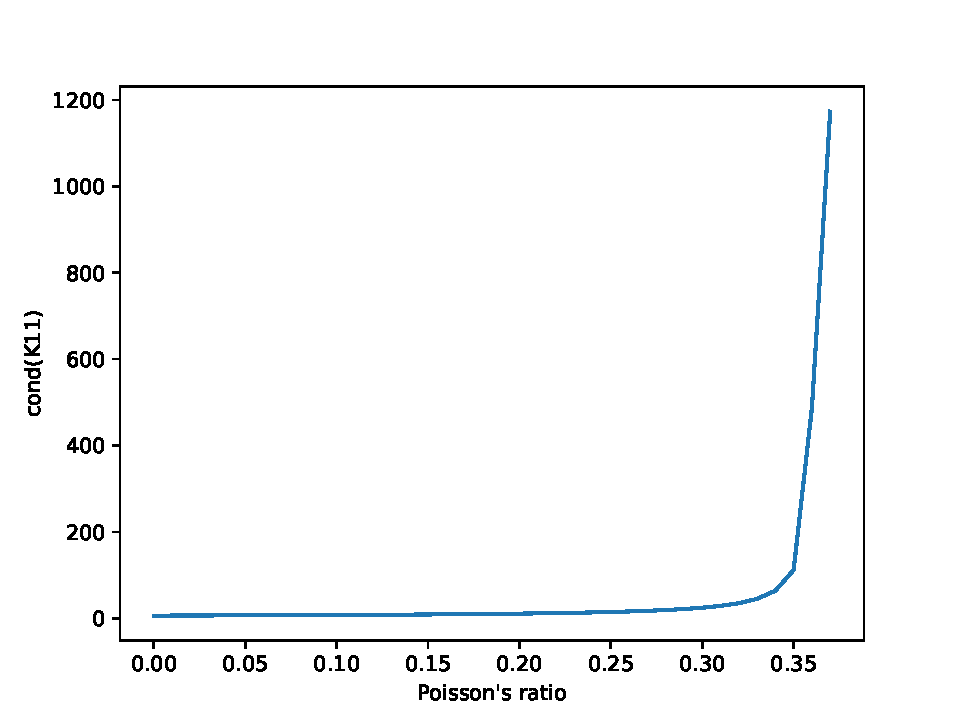
\includegraphics[height = 0.37 \linewidth]{exp/cond.pdf}}
  \subcaptionbox{平均误差 \label{fig:mean}}{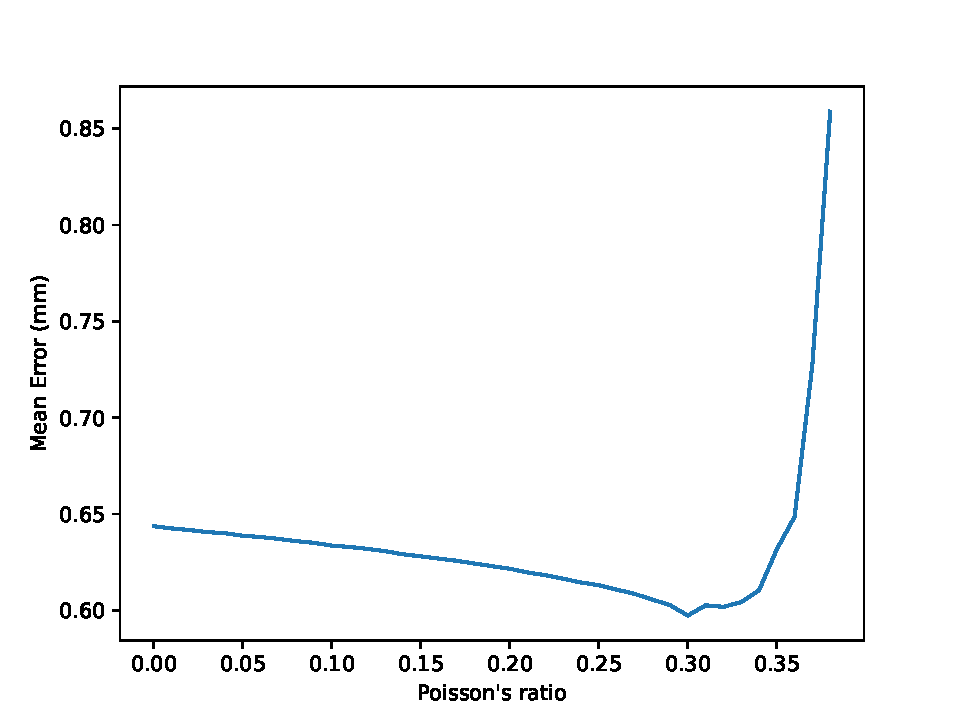
\includegraphics[height = 0.37 \linewidth]{exp/mean.pdf}}
  \subcaptionbox{\SI{95}{\percent} 误差 \label{fig:95}}{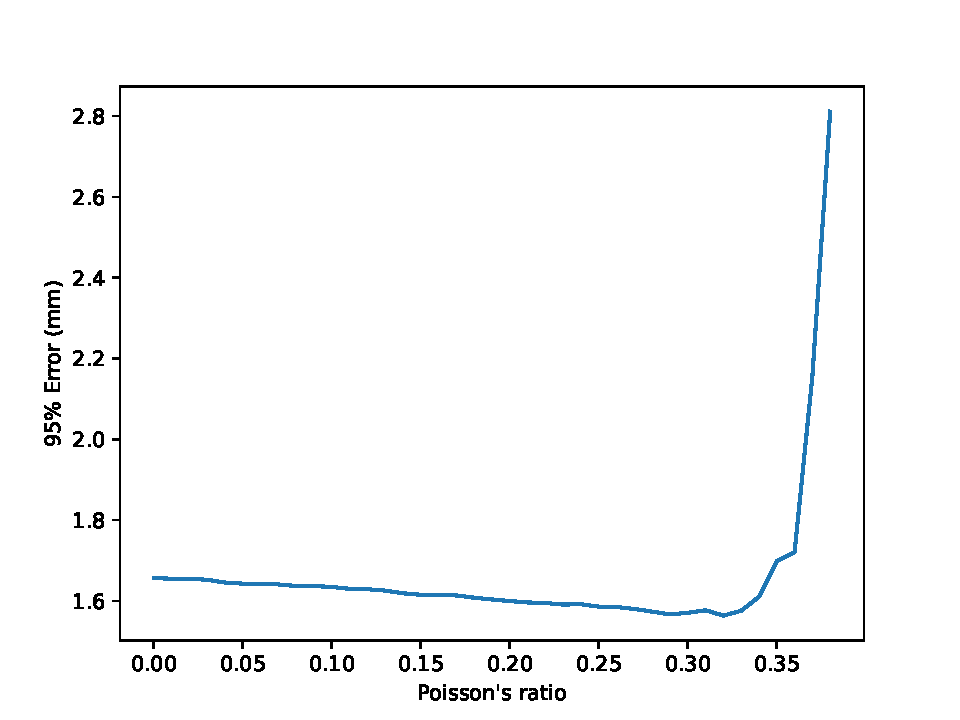
\includegraphics[height = 0.37 \linewidth]{exp/95.pdf}}
  \subcaptionbox{最大误差 \label{fig:max}}{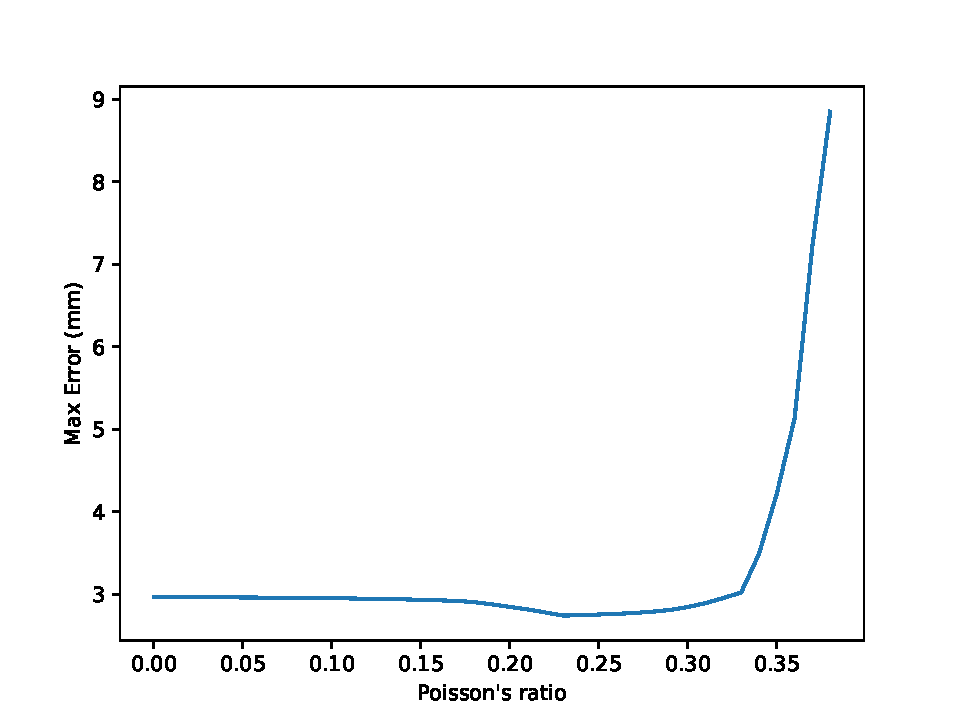
\includegraphics[height = 0.37 \linewidth]{exp/max.pdf}}
  \caption{泊松比对结果的影响}
\end{figure}

\section{准确性}
\label{sec:accuracy}

我们针对 10 组真实的临床案例数据进行了详尽的测试。
每组数据均包括术前及术后约一年时的 CT 影像。
为了定量分析我们方法的准确性,我们选取了每组数据中我们关心的区域(如图 \ref{fig:120056} 所示为例),在这些区域内,我们统计了预测的术后面部模型每个顶点到真实术后模型表面的最短距离。
各项指标的统计结果见表 \ref{tab:results}。

图 \ref{fig:120056} 显示了一例具体数据的可视化效果。
手术内容包括下颌角 + 外板打磨、颧骨磨低,以及颏部水平截骨。
在预测结果中,不同的颜色标识了相对于真实术后模型的误差程度。
从图中可以清晰看出,本研究所提出的方法成功预测了下巴的前移和脸颊的收缩。
图 \ref{fig:113286} 则展示了另一例可视化结果,该手术涉及下颌角 + 外板打磨、颧骨截骨降低。
通过预测结果与真实术后外形的对比,可以表明本方法具备较高精度地预测术后面部形状的能力。

\begin{table}
  \centering
  \caption{预测结果统计}
  \label{tab:results}
  \sisetup{
    table-format = 1.2,
  }
  \begin{tabular}{c S S S S}
    \toprule
    ID   & {平均误差 / \unit{\milli\meter}} & {标准差 / \unit{\milli\meter}} & {\SI{95}{\percent} 置信区间 / \unit{\milli\meter}} & {最大误差 / \unit{\milli\meter}} \\
    \midrule
    0    & 0.60                             & 0.65                           & 2.10                                               & 5.32                             \\
    1    & 0.73                             & 0.55                           & 1.52                                               & 4.17                             \\
    2    & 0.91                             & 0.89                           & 2.86                                               & 6.48                             \\
    3    & 0.70                             & 0.85                           & 2.75                                               & 4.96                             \\
    4    & 0.29                             & 0.39                           & 1.13                                               & 3.10                             \\
    5    & 0.62                             & 0.67                           & 2.01                                               & 4.56                             \\
    6    & 0.87                             & 1.08                           & 3.51                                               & 5.57                             \\
    7    & 0.72                             & 0.66                           & 2.10                                               & 4.77                             \\
    8    & 0.57                             & 0.51                           & 1.70                                               & 3.64                             \\
    9    & 0.61                             & 0.48                           & 1.59                                               & 2.68                             \\
    平均 & 0.66                             & 0.67                           & 2.13                                               & 4.53                             \\
    \bottomrule
  \end{tabular}
\end{table}

\section{计算效率}

我们基于 MeshTaichi 框架 \cite{yuMeshTaichiCompilerEfficient2022} 实现了本文提出的方法。
MeshTaichi 能够并行化加速网格操作,从而提高计算效率。
我们在一台配备有 Intel Core i9-13900HX CPU 的计算机上进行了测试。
对于每位患者,数据预处理的步骤仅需执行一次,花费时间约为 \SI{5}{\minute}。
在评估手术规划的效果时,每一次对术后面部进行预测的过程仅需要大约 \SI{15}{\second}。

\begin{figure}[p]
  \centering
  \begin{tblr}{Q[c,m] Q[c,m] Q[c,m]}
    \SetCell[r=2]{c} 术前                                                   &
    \includegraphics[height = 0.27 \textwidth]{120056/pre-skull-front.pdf}  &
    \includegraphics[height = 0.27 \textwidth]{120056/pre-skull-lateral.pdf}  \\
                                                                            &
    \includegraphics[height = 0.27 \textwidth]{120056/pre-face-front.pdf}   &
    \includegraphics[height = 0.27 \textwidth]{120056/pre-face-lateral.pdf}   \\
    \SetCell[r=2]{c} 术后                                                   &
    \includegraphics[height = 0.27 \textwidth]{120056/post-skull-front.pdf} &
    \includegraphics[height = 0.27 \textwidth]{120056/post-skull-lateral.pdf} \\
                                                                            &
    \includegraphics[height = 0.27 \textwidth]{120056/post-face-front.pdf}  &
    \includegraphics[height = 0.27 \textwidth]{120056/post-face-lateral.pdf}  \\
    预测                                                                    &
    \includegraphics[height = 0.27 \textwidth]{120056/predict-front.pdf}    &
    \includegraphics[height = 0.27 \textwidth]{120056/predict-lateral.pdf}
  \end{tblr}
  \caption{手术前后对比分析 (下颌角 + 外板打磨、颧骨磨低、颏部水平截骨)}
  \label{fig:120056}
\end{figure}

\begin{figure}[p]
  \centering
  \begin{tblr}{Q[c,m] Q[c,m] Q[c,m]}
    \SetCell[r=2]{c} 术前                                                   &
    \includegraphics[height = 0.27 \textwidth]{113286/pre-skull-front.pdf}  &
    \includegraphics[height = 0.27 \textwidth]{113286/pre-skull-lateral.pdf}  \\
                                                                            &
    \includegraphics[height = 0.27 \textwidth]{113286/pre-face-front.pdf}   &
    \includegraphics[height = 0.27 \textwidth]{113286/pre-face-lateral.pdf}   \\
    \SetCell[r=2]{c} 术后                                                   &
    \includegraphics[height = 0.27 \textwidth]{113286/post-skull-front.pdf} &
    \includegraphics[height = 0.27 \textwidth]{113286/post-skull-lateral.pdf} \\
                                                                            &
    \includegraphics[height = 0.27 \textwidth]{113286/post-face-front.pdf}  &
    \includegraphics[height = 0.27 \textwidth]{113286/post-face-lateral.pdf}  \\
    预测                                                                    &
    \includegraphics[height = 0.27 \textwidth]{113286/predict-front.pdf}    &
    \includegraphics[height = 0.27 \textwidth]{113286/predict-lateral.pdf}
  \end{tblr}
  \caption{手术前后对比分析 (下颌角 + 外板打磨、颧骨截骨降低)}
  \label{fig:113286}
\end{figure}
